\documentclass[oneside]{book}

% Packages required by doxygen
\usepackage{fixltx2e}
\usepackage{calc}
\usepackage{doxygen}
\usepackage[export]{adjustbox} % also loads graphicx
\usepackage{graphicx}
\usepackage[utf8]{inputenc}
\usepackage{makeidx}
\usepackage{multicol}
\usepackage{multirow}
\PassOptionsToPackage{warn}{textcomp}
\usepackage{textcomp}
\usepackage[nointegrals]{wasysym}
\usepackage[table]{xcolor}

% Font selection
\usepackage[T1]{fontenc}
\usepackage[scaled=.90]{helvet}
\usepackage{courier}
\usepackage{amssymb}
\usepackage{sectsty}
\renewcommand{\familydefault}{\sfdefault}
\allsectionsfont{%
  \fontseries{bc}\selectfont%
  \color{darkgray}%
}
\renewcommand{\DoxyLabelFont}{%
  \fontseries{bc}\selectfont%
  \color{darkgray}%
}
\newcommand{\+}{\discretionary{\mbox{\scriptsize$\hookleftarrow$}}{}{}}

% Page & text layout
\usepackage{geometry}
\geometry{%
  a4paper,%
  top=2.5cm,%
  bottom=2.5cm,%
  left=2.5cm,%
  right=2.5cm%
}
\tolerance=750
\hfuzz=15pt
\hbadness=750
\setlength{\emergencystretch}{15pt}
\setlength{\parindent}{0cm}
\setlength{\parskip}{3ex plus 2ex minus 2ex}
\makeatletter
\renewcommand{\paragraph}{%
  \@startsection{paragraph}{4}{0ex}{-1.0ex}{1.0ex}{%
    \normalfont\normalsize\bfseries\SS@parafont%
  }%
}
\renewcommand{\subparagraph}{%
  \@startsection{subparagraph}{5}{0ex}{-1.0ex}{1.0ex}{%
    \normalfont\normalsize\bfseries\SS@subparafont%
  }%
}
\makeatother

% Headers & footers
\usepackage{fancyhdr}
\pagestyle{fancyplain}
\fancyhead[LE]{\fancyplain{}{\bfseries\thepage}}
\fancyhead[CE]{\fancyplain{}{}}
\fancyhead[RE]{\fancyplain{}{\bfseries\leftmark}}
\fancyhead[LO]{\fancyplain{}{\bfseries\rightmark}}
\fancyhead[CO]{\fancyplain{}{}}
\fancyhead[RO]{\fancyplain{}{\bfseries\thepage}}
\fancyfoot[LE]{\fancyplain{}{}}
\fancyfoot[CE]{\fancyplain{}{}}
\fancyfoot[RE]{\fancyplain{}{\bfseries\scriptsize Generated by Doxygen }}
\fancyfoot[LO]{\fancyplain{}{\bfseries\scriptsize Generated by Doxygen }}
\fancyfoot[CO]{\fancyplain{}{}}
\fancyfoot[RO]{\fancyplain{}{}}
\renewcommand{\footrulewidth}{0.4pt}
\renewcommand{\chaptermark}[1]{%
  \markboth{#1}{}%
}
\renewcommand{\sectionmark}[1]{%
  \markright{\thesection\ #1}%
}

% Indices & bibliography
\usepackage{natbib}
\usepackage[titles]{tocloft}
\setcounter{tocdepth}{3}
\setcounter{secnumdepth}{5}
\makeindex

% Hyperlinks (required, but should be loaded last)
\usepackage{ifpdf}
\ifpdf
  \usepackage[pdftex,pagebackref=true]{hyperref}
\else
  \usepackage[ps2pdf,pagebackref=true]{hyperref}
\fi
\hypersetup{%
  colorlinks=true,%
  linkcolor=blue,%
  citecolor=blue,%
  unicode%
}

% Custom commands
\newcommand{\clearemptydoublepage}{%
  \newpage{\pagestyle{empty}\cleardoublepage}%
}

\usepackage{caption}
\captionsetup{labelsep=space,justification=centering,font={bf},singlelinecheck=off,skip=4pt,position=top}

%===== C O N T E N T S =====

\begin{document}

% Titlepage & ToC
\hypersetup{pageanchor=false,
             bookmarksnumbered=true,
             pdfencoding=unicode
            }
\pagenumbering{alph}
\begin{titlepage}
\vspace*{7cm}
\begin{center}%
{\Large Snake \\[1ex]\large 1 }\\
\vspace*{1cm}
{\large Generated by Doxygen 1.8.14}\\
\end{center}
\end{titlepage}
\clearemptydoublepage
\pagenumbering{roman}
\tableofcontents
\clearemptydoublepage
\pagenumbering{arabic}
\hypersetup{pageanchor=true}

%--- Begin generated contents ---
\chapter{Namespace Index}
\section{Packages}
Here are the packages with brief descriptions (if available)\+:\begin{DoxyCompactList}
\item\contentsline{section}{\mbox{\hyperlink{namespace_snake}{Snake}} }{\pageref{namespace_snake}}{}
\end{DoxyCompactList}

\chapter{Hierarchical Index}
\section{Class Hierarchy}
This inheritance list is sorted roughly, but not completely, alphabetically\+:\begin{DoxyCompactList}
\item Tk\begin{DoxyCompactList}
\item \contentsline{section}{Snake.\+Game}{\pageref{class_snake_1_1_game}}{}
\end{DoxyCompactList}
\end{DoxyCompactList}

\chapter{Class Index}
\section{Class List}
Here are the classes, structs, unions and interfaces with brief descriptions\+:\begin{DoxyCompactList}
\item\contentsline{section}{\mbox{\hyperlink{class_esp_server}{Esp\+Server}} }{\pageref{class_esp_server}}{}
\end{DoxyCompactList}

\chapter{Namespace Documentation}
\hypertarget{namespace_snake}{}\section{Snake Namespace Reference}
\label{namespace_snake}\index{Snake@{Snake}}
\subsection*{Classes}
\begin{DoxyCompactItemize}
\item 
class \mbox{\hyperlink{class_snake_1_1_game}{Game}}
\end{DoxyCompactItemize}
\subsection*{Functions}
\begin{DoxyCompactItemize}
\item 
def \mbox{\hyperlink{namespace_snake_a91223592dfcc9c233f9d7c5b16809456}{createfield}} ()
\item 
def \mbox{\hyperlink{namespace_snake_a8f6d4da01109c97d36f9a18d5a0bb0b3}{firststart}} ()
\end{DoxyCompactItemize}
\subsection*{Variables}
\begin{DoxyCompactItemize}
\item 
\mbox{\Hypertarget{namespace_snake_a10cc7da73d7488752c4a8222135707a1}\label{namespace_snake_a10cc7da73d7488752c4a8222135707a1}} 
{\bfseries s} = socket.\+socket()
\item 
\mbox{\Hypertarget{namespace_snake_a26464c0ce15e8a65c02d8b1d0e077ea4}\label{namespace_snake_a26464c0ce15e8a65c02d8b1d0e077ea4}} 
int {\bfseries size} = 25
\item 
\mbox{\Hypertarget{namespace_snake_a3aef21f736569d8b66197f0e7397c801}\label{namespace_snake_a3aef21f736569d8b66197f0e7397c801}} 
bool {\bfseries feedcollision} = False
\item 
\mbox{\Hypertarget{namespace_snake_a3066d1fa56dad61e41bb50f0f85eb79a}\label{namespace_snake_a3066d1fa56dad61e41bb50f0f85eb79a}} 
int {\bfseries length} = 1
\item 
\mbox{\Hypertarget{namespace_snake_a27bdeea7ec49893ec1aa7f5e0cc2967e}\label{namespace_snake_a27bdeea7ec49893ec1aa7f5e0cc2967e}} 
{\bfseries direction} = randint(1,4)
\item 
\mbox{\Hypertarget{namespace_snake_a7fab8854941bcbd85234bec6d4879176}\label{namespace_snake_a7fab8854941bcbd85234bec6d4879176}} 
int {\bfseries xx} = 8
\item 
\mbox{\Hypertarget{namespace_snake_a027467285b250e9abb387c2c1326771c}\label{namespace_snake_a027467285b250e9abb387c2c1326771c}} 
int {\bfseries yy} = 8
\item 
\mbox{\Hypertarget{namespace_snake_ab110474976787cf3ccef734d19a75630}\label{namespace_snake_ab110474976787cf3ccef734d19a75630}} 
list {\bfseries feedpoint} = \mbox{[}randint(1,16),randint(1,16)\mbox{]}
\item 
\mbox{\Hypertarget{namespace_snake_a5007979b981a90f08d3775ef8714c84c}\label{namespace_snake_a5007979b981a90f08d3775ef8714c84c}} 
list {\bfseries xcoordinate} = \mbox{[}xx\mbox{]}
\item 
\mbox{\Hypertarget{namespace_snake_aab72c72a638d0b108981f93348891b18}\label{namespace_snake_aab72c72a638d0b108981f93348891b18}} 
list {\bfseries ycoordinate} = \mbox{[}yy\mbox{]}
\item 
\mbox{\Hypertarget{namespace_snake_a0bc14678957b8b5a8dfac41d8e647041}\label{namespace_snake_a0bc14678957b8b5a8dfac41d8e647041}} 
bool {\bfseries lost} = False
\item 
\mbox{\Hypertarget{namespace_snake_aa277acac43eb5cd735f12bf81f3e94bb}\label{namespace_snake_aa277acac43eb5cd735f12bf81f3e94bb}} 
int {\bfseries score} = 0
\item 
\mbox{\Hypertarget{namespace_snake_ab2b5f6ed36de41b8f318733bc26b93ae}\label{namespace_snake_ab2b5f6ed36de41b8f318733bc26b93ae}} 
int {\bfseries highscore} = 0
\item 
\mbox{\Hypertarget{namespace_snake_ac11d51dc9d52703ce138d3b42c094a18}\label{namespace_snake_ac11d51dc9d52703ce138d3b42c094a18}} 
{\bfseries game} = \mbox{\hyperlink{class_snake_1_1_game}{Game}}()
\end{DoxyCompactItemize}


\subsection{Detailed Description}
\begin{DoxyVerb}Informatik Projekt 2018
Thema:  Snake
Erstellt von: Adrian Bergen(4228620), Lukas Hansen(4463302), Fanziska Bollhorst (4463145)

Am Anfang werden die benötigten librarys importiert. Tkinter für die GUI,
Socket für die Kommunikation, Random für zufällige Zahlen.

Außerdem werden die für das Spiel benötigten Anfangsvariabeln erstellt.
size: Größe der Quadrate, auf den das Spielfeld gezeichnet wird.
feedcollision: Am Anfang kollidiert die Schlange nicht mit einem Punkt
length: Länge der Schlange, vergrößert sich beim Aufsammeln eines Punktes
direction: Zahlen von 1-4, sie stehen für die jeweilige Richtung.
Dabei wird direction von Arduino gesteuert.
xx und yy: Reine Anfangskoordinaten der Schlange auf dem Feld.
(Das Feld ist 16x16)
x/ycoordinate: xx und yy werden in jeweils einem Array gepackt.
Später zeigt das Array die Punkte aller Schlangenpunkte.
(Also länge des Arrays =Länge der Schlange)
lost: Ist standartmäßig nicht True
score/ Highscore: Ist am Anfang 0
\end{DoxyVerb}
 

\subsection{Function Documentation}
\mbox{\Hypertarget{namespace_snake_a91223592dfcc9c233f9d7c5b16809456}\label{namespace_snake_a91223592dfcc9c233f9d7c5b16809456}} 
\index{Snake@{Snake}!createfield@{createfield}}
\index{createfield@{createfield}!Snake@{Snake}}
\subsubsection{\texorpdfstring{createfield()}{createfield()}}
{\footnotesize\ttfamily def Snake.\+createfield (\begin{DoxyParamCaption}{ }\end{DoxyParamCaption})}

\begin{DoxyVerb}Hier wird das erste mal das richtige Spielfeld erstellt. Es wird der Spielername übernommen
und nach oben links gesetzt, Score und Highscore nach oben rechts. Das Startfenster wird gelöscht.
Der Ticker wird zum ersten mal gestartet. Der Feedpoint wird gesetzt.
\end{DoxyVerb}
 \mbox{\Hypertarget{namespace_snake_a8f6d4da01109c97d36f9a18d5a0bb0b3}\label{namespace_snake_a8f6d4da01109c97d36f9a18d5a0bb0b3}} 
\index{Snake@{Snake}!firststart@{firststart}}
\index{firststart@{firststart}!Snake@{Snake}}
\subsubsection{\texorpdfstring{firststart()}{firststart()}}
{\footnotesize\ttfamily def Snake.\+firststart (\begin{DoxyParamCaption}{ }\end{DoxyParamCaption})}

\begin{DoxyVerb}Wird das Spiel gestartet, erscheint ein Fenster mit Namenseingabe und einem Startknopf.
Durch diesen Startknopf startet sich das Spiel.
\end{DoxyVerb}
 
\chapter{Class Documentation}
\hypertarget{class_snake_1_1_game}{}\section{Snake.\+Game Class Reference}
\label{class_snake_1_1_game}\index{Snake.\+Game@{Snake.\+Game}}
Inheritance diagram for Snake.\+Game\+:\begin{figure}[H]
\begin{center}
\leavevmode
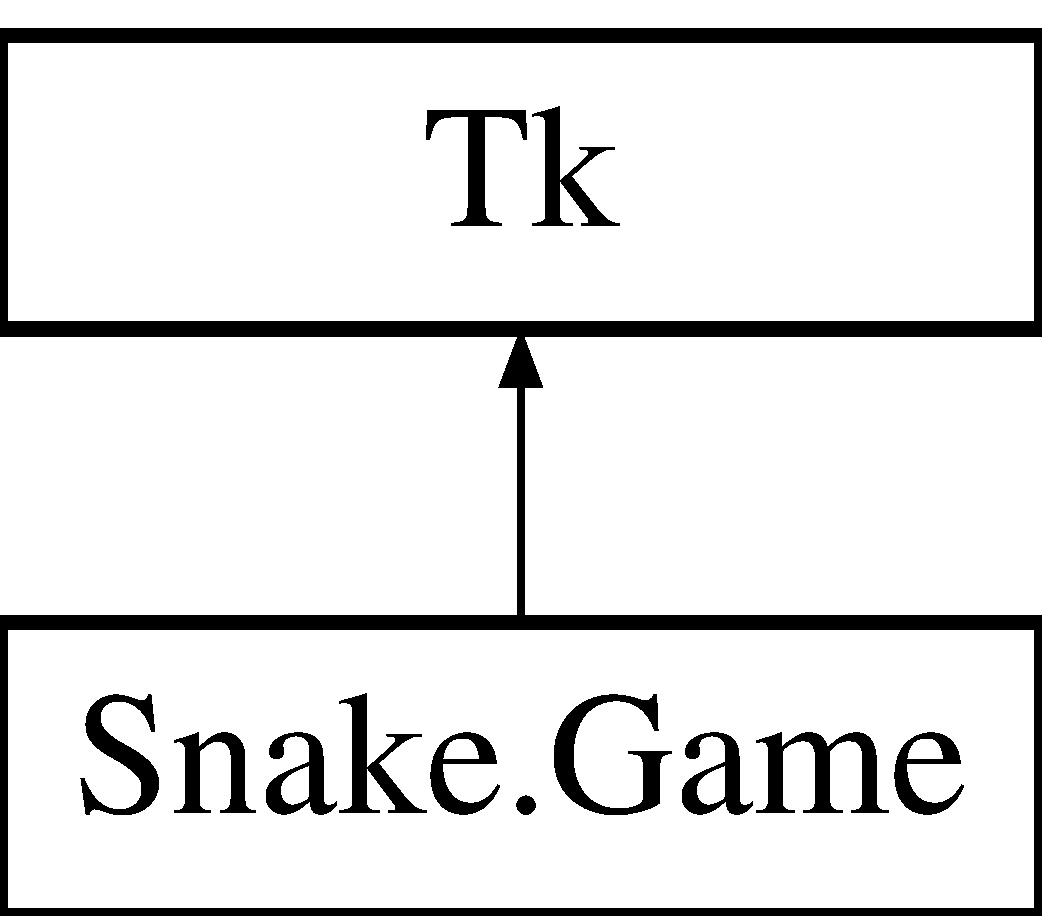
\includegraphics[height=2.000000cm]{class_snake_1_1_game}
\end{center}
\end{figure}
\subsection*{Public Member Functions}
\begin{DoxyCompactItemize}
\item 
def \mbox{\hyperlink{class_snake_1_1_game_aedca2341f309daf9d1fdd1c1b5fbbb74}{createbutton}} (self)
\item 
def \mbox{\hyperlink{class_snake_1_1_game_a7b60758212d640631d9fdb6d4f7af472}{ticker}} (self)
\item 
def \mbox{\hyperlink{class_snake_1_1_game_aee9e8a04fb8c7d56f3b3230fa4d8a66b}{drawsnake}} (self)
\item 
def \mbox{\hyperlink{class_snake_1_1_game_a98cef3415a4d544424cd9bc57e348ab7}{feedpoint}} (self)
\item 
def \mbox{\hyperlink{class_snake_1_1_game_a47967ef289465a984d6c86b34ead527e}{createfeedpoint}} (self)
\item 
def \mbox{\hyperlink{class_snake_1_1_game_a280b6182e187f4b13756abbc8776bfc0}{collisions}} (self)
\item 
def \mbox{\hyperlink{class_snake_1_1_game_a30c722d4cdac2ba08f691a89a31e3306}{doastep}} (self)
\item 
def \mbox{\hyperlink{class_snake_1_1_game_a5cdcfd6cdea9949bfe5005cb602c68d4}{restart}} (self)
\item 
def \mbox{\hyperlink{class_snake_1_1_game_aebc0cbe1082bdba9f171f075ad8f6693}{receivearduino}} (self)
\end{DoxyCompactItemize}


\subsection{Member Function Documentation}
\mbox{\Hypertarget{class_snake_1_1_game_a280b6182e187f4b13756abbc8776bfc0}\label{class_snake_1_1_game_a280b6182e187f4b13756abbc8776bfc0}} 
\index{Snake\+::\+Game@{Snake\+::\+Game}!collisions@{collisions}}
\index{collisions@{collisions}!Snake\+::\+Game@{Snake\+::\+Game}}
\subsubsection{\texorpdfstring{collisions()}{collisions()}}
{\footnotesize\ttfamily def Snake.\+Game.\+collisions (\begin{DoxyParamCaption}\item[{}]{self }\end{DoxyParamCaption})}

\begin{DoxyVerb}Diese Funktion checkt die Kollision mit den Spielfeldrändern und der Schlange selber. 
Passiert dies, wird lost=True gesetzt und der Ticker läuft im nächsten
Durchgang nicht weiter.
\end{DoxyVerb}
 \mbox{\Hypertarget{class_snake_1_1_game_aedca2341f309daf9d1fdd1c1b5fbbb74}\label{class_snake_1_1_game_aedca2341f309daf9d1fdd1c1b5fbbb74}} 
\index{Snake\+::\+Game@{Snake\+::\+Game}!createbutton@{createbutton}}
\index{createbutton@{createbutton}!Snake\+::\+Game@{Snake\+::\+Game}}
\subsubsection{\texorpdfstring{createbutton()}{createbutton()}}
{\footnotesize\ttfamily def Snake.\+Game.\+createbutton (\begin{DoxyParamCaption}\item[{}]{self }\end{DoxyParamCaption})}

\begin{DoxyVerb}Hier wird ein Knopf erstellt, nachdem man bei dem Spiel verliert.
Dieser Knopf dient dazu das Spiel neu zu starten (Aufrufen der Funktion "restart").
Des Weiteren wird ein Textfeld erstellt. Dieses benachrichtigt dich, dass du verloren hast.
\end{DoxyVerb}
 \mbox{\Hypertarget{class_snake_1_1_game_a47967ef289465a984d6c86b34ead527e}\label{class_snake_1_1_game_a47967ef289465a984d6c86b34ead527e}} 
\index{Snake\+::\+Game@{Snake\+::\+Game}!createfeedpoint@{createfeedpoint}}
\index{createfeedpoint@{createfeedpoint}!Snake\+::\+Game@{Snake\+::\+Game}}
\subsubsection{\texorpdfstring{createfeedpoint()}{createfeedpoint()}}
{\footnotesize\ttfamily def Snake.\+Game.\+createfeedpoint (\begin{DoxyParamCaption}\item[{}]{self }\end{DoxyParamCaption})}

\begin{DoxyVerb}Hier wird der feedpoint generiert. Es passiert zufällig auf dem Spielfeld. Es ist darauf
zu achten, dass der Punkt nicht auf der Schlange generiert wird, andernfalls wird ein
neuer Punkt generiert.
\end{DoxyVerb}
 \mbox{\Hypertarget{class_snake_1_1_game_a30c722d4cdac2ba08f691a89a31e3306}\label{class_snake_1_1_game_a30c722d4cdac2ba08f691a89a31e3306}} 
\index{Snake\+::\+Game@{Snake\+::\+Game}!doastep@{doastep}}
\index{doastep@{doastep}!Snake\+::\+Game@{Snake\+::\+Game}}
\subsubsection{\texorpdfstring{doastep()}{doastep()}}
{\footnotesize\ttfamily def Snake.\+Game.\+doastep (\begin{DoxyParamCaption}\item[{}]{self }\end{DoxyParamCaption})}

\begin{DoxyVerb}Bestimme die neuen Koordinaten von Snake, abhängig von der momentanten Richtung.
\end{DoxyVerb}
 \mbox{\Hypertarget{class_snake_1_1_game_aee9e8a04fb8c7d56f3b3230fa4d8a66b}\label{class_snake_1_1_game_aee9e8a04fb8c7d56f3b3230fa4d8a66b}} 
\index{Snake\+::\+Game@{Snake\+::\+Game}!drawsnake@{drawsnake}}
\index{drawsnake@{drawsnake}!Snake\+::\+Game@{Snake\+::\+Game}}
\subsubsection{\texorpdfstring{drawsnake()}{drawsnake()}}
{\footnotesize\ttfamily def Snake.\+Game.\+drawsnake (\begin{DoxyParamCaption}\item[{}]{self }\end{DoxyParamCaption})}

\begin{DoxyVerb}Zuerst wird geprüft, ob die Schlange mit einem Punkt (Futter) kollidiert.
Anschließend wird das Array x/ycoordinate um die jeweilige NEUE x/y Koordinate erweitert.
Bei collisions wird die Kollision mit der Schlange selber, sowie den Wänden geprüft.
doastep verändert xx und yy, jenachdem welche "direction" die Schlange gerade hat.
Als nächstes wird der neue Kopf der Schlange gezeichnet, anschließend wird
hinten wieder die Spielfeldfarbe gezeichnet - Eine Schlange entsteht.
Da die Länge der Schlange von Punktekollisionen gesteuert wird, muss sich das
Array darauf anpassen, so wächst die Schlange tatsächlich auch.
\end{DoxyVerb}
 \mbox{\Hypertarget{class_snake_1_1_game_a98cef3415a4d544424cd9bc57e348ab7}\label{class_snake_1_1_game_a98cef3415a4d544424cd9bc57e348ab7}} 
\index{Snake\+::\+Game@{Snake\+::\+Game}!feedpoint@{feedpoint}}
\index{feedpoint@{feedpoint}!Snake\+::\+Game@{Snake\+::\+Game}}
\subsubsection{\texorpdfstring{feedpoint()}{feedpoint()}}
{\footnotesize\ttfamily def Snake.\+Game.\+feedpoint (\begin{DoxyParamCaption}\item[{}]{self }\end{DoxyParamCaption})}

\begin{DoxyVerb}Kollidiert der Schlangenkopf mit den x und y Koordinaten des feedpoints?
Dann verändert sich der Score, die Schlange wächst um 1, ein neuer Punkt wird erstellt.
\end{DoxyVerb}
 \mbox{\Hypertarget{class_snake_1_1_game_aebc0cbe1082bdba9f171f075ad8f6693}\label{class_snake_1_1_game_aebc0cbe1082bdba9f171f075ad8f6693}} 
\index{Snake\+::\+Game@{Snake\+::\+Game}!receivearduino@{receivearduino}}
\index{receivearduino@{receivearduino}!Snake\+::\+Game@{Snake\+::\+Game}}
\subsubsection{\texorpdfstring{receivearduino()}{receivearduino()}}
{\footnotesize\ttfamily def Snake.\+Game.\+receivearduino (\begin{DoxyParamCaption}\item[{}]{self }\end{DoxyParamCaption})}

\begin{DoxyVerb}Empfange vom Arduino die Richtungsdaten (String). Man unterscheidet zwischen
'u', 're', 'l', 'o' für die jeweiligen Richtungen. Es ist darauf zu achten,
dass die Schlange keine 180° Wende machen kann.
\end{DoxyVerb}
 \mbox{\Hypertarget{class_snake_1_1_game_a5cdcfd6cdea9949bfe5005cb602c68d4}\label{class_snake_1_1_game_a5cdcfd6cdea9949bfe5005cb602c68d4}} 
\index{Snake\+::\+Game@{Snake\+::\+Game}!restart@{restart}}
\index{restart@{restart}!Snake\+::\+Game@{Snake\+::\+Game}}
\subsubsection{\texorpdfstring{restart()}{restart()}}
{\footnotesize\ttfamily def Snake.\+Game.\+restart (\begin{DoxyParamCaption}\item[{}]{self }\end{DoxyParamCaption})}

\begin{DoxyVerb}Wenn man verliert, muss das Spiel neu aufgesetzt werden.
Das Spielfeld wird neu gezeichnet, ein neuer Highscore wird bestimmt. 
Es erscheint ein Text, dass man verloren hat und die Variabeln werden
zurückgesetzt (z.B. die Koordinaten). Der Ticker wird neugestartet.
\end{DoxyVerb}
 \mbox{\Hypertarget{class_snake_1_1_game_a7b60758212d640631d9fdb6d4f7af472}\label{class_snake_1_1_game_a7b60758212d640631d9fdb6d4f7af472}} 
\index{Snake\+::\+Game@{Snake\+::\+Game}!ticker@{ticker}}
\index{ticker@{ticker}!Snake\+::\+Game@{Snake\+::\+Game}}
\subsubsection{\texorpdfstring{ticker()}{ticker()}}
{\footnotesize\ttfamily def Snake.\+Game.\+ticker (\begin{DoxyParamCaption}\item[{}]{self }\end{DoxyParamCaption})}

\begin{DoxyVerb}Das Herz des Spiels. Ticker ruft sich alle 0,6 Sekunden rekursiv mithilfe einer after-Funktion wieder auf.
Mit receivearduino wird die direction von Snake empfangen.
Die Funktion ruft sich nicht wieder auf, wenn man verloren hat. Stattdessen hört das Spiel auf und der
Neustartbutton wird erstellt.
\end{DoxyVerb}
 

The documentation for this class was generated from the following file\+:\begin{DoxyCompactItemize}
\item 
Snake.\+py\end{DoxyCompactItemize}

%--- End generated contents ---

% Index
\backmatter
\newpage
\phantomsection
\clearemptydoublepage
\addcontentsline{toc}{chapter}{Index}
\printindex

\end{document}
